\documentclass[letterpaper, 12pt]{report}
\usepackage[spanish]{babel}
\usepackage[latin1]{inputenc}
%\usepackage[T1]{fontenc}
\usepackage[Sonny]{fncychap}
\usepackage{fullpage}
%\usepackage{algorithm}

\bibliographystyle{plain}
\setcounter{secnumdepth}{3}
\setcounter{tocdepth}{3}
\pagenumbering{roman}

\title{Desarrollo de un Software Libre para la interpretaci�n de ondas cerebrales}
\author{Carlos Antonio Bulnes Dom�nguez}

\begin{document}

\newcounter{rom}


\begin{titlepage}
\maketitle
\end{titlepage}\newpage\thispagestyle{plain}

\addtocounter{rom}{1}\setcounter{page}{2}~
\newpage\thispagestyle{plain}\setcounter{page}{3}

\tableofcontents

\newpage\thispagestyle{plain}~
\clearpage
\pagenumbering{arabic}

\chapter*{Introducci�n}
\markboth{\MakeUppercase{Introducci�n}}{}
\addcontentsline{toc}{chapter}{Introducci�n}

\indent El trabajo presentado describe la realizaci�n de un software libre desarrollado con ROS para ser utilizado con un lector de ondas cerebrales. El nuevo software tiene como objetivo la lectura, graficaci�n y registro de los datos que reciba a trav�s de la plataforma ROS. Durante la investigaci�n se encontr� que ya exist�a un software similar, sin embargo este resultaba muy lento lo que provocaba que la informaci�n en pantalla no fuera fiable. El software resultante en este trabajo tiene como objetivo resolver ese problema, es por eso que, como se explicar� en cap�tulos posteriores, se escogi� integrarlo a ROS.
\\ \indent El nuevo software permitir� controlar el momento en que se quiera Ejecutar, Pausar y Detener la recepci�n de la informaci�n, estas acciones no afectar�n al programa que env�a los datos pues solo afecta de forma visual al programa receptor para que el usuario tenga control de que quiere ver y en que momentos. Adicionalmente cuenta con la funcionalidad de visualizar y crear un registro de todas las se�ales que se reciban mientras el software se encuentre en modo de ``reproducci�n''. La visualizaci�n es e tiempo real mientras que la generaci�n del registro se genera cuando se presiona ``detener'' y crear� un archivo en disco duro con el nombre que se haya ingresado as� como la fecha y hora de creaci�n de este, dicho archivo permitir� al usuario consultarlo en cualquier momento independientemente de que el software se encuentre en ejecuci�n o no.\newpage\cleardoublepage
\chapter*{Justificaci�n}
\markboth{\MakeUppercase{Justificaci�n}}{}
\addcontentsline{toc}{chapter}{Justificaci�n}


La necesidad de la creaci�n de un software libre para la lectura de las ondas cerebrales surge debido a la escaza variedad de programas dedicados a dicha tarea actualmente, donde es el mismo creador del dispositivo f�sico el que te proporciona el software, el cual, ya cuenta con funciones y operaciones definidas por el fabricante.
\\ \indent
En la actualidad los proyectos de investigaci�n requieren interactuar m�s con la informaci�n que obtienen con los dispositivos lectores de ondas cerebrales, y como ya se mencion�, las alternativas actuales se encuentran limitadas, se propone entonces un proyecto de c�digo libre en el cual, partiendo del software desarrollado en este trabajo, los desarrolladores futuros sean capaces de complementarlo e implementarlos a sus necesidades espec�ficas.
\newpage\cleardoublepage
\section*{Hip�tesis}
\markboth{\MakeUppercase{Hip�tesis}}{}
\addcontentsline{toc}{section}{Hip�tesis}
El software desarrollado leer� las se�ales de un EEG y las graficar�. Las gr�ficas ser�n en tiempo real, las cuales estar�n monitoreando las se�ales recibidas en una relaci�n frecuencia-tiempo (como lo hace un Osciloscopio electr�nico). Adem�s se podr�n obtener dichos datos en valores num�ricos para que as� el software pueda comunicarse con otras herramientas.
\newpage\cleardoublepage
\section*{Objetivos}
\markboth{\MakeUppercase{Objetivos}}{}
\addcontentsline{toc}{section}{Objetivos}

\subsection*{Objetivo General}
\markboth{\MakeUppercase{Objetivo General}}{}
\addcontentsline{toc}{subsection}{Objetivo General}
%Crear un software libre capaz de interpretar las se�ales de un EEG para que puedan ser usadas por medio de herramientas externas.
Crear un software libre capaz de leer y graficar en tiempo real a trav�s de la plataforma ROS las se�ales enviadas por el Emotiv EPOC, las cuales son interpretadas por un software libre llamado emokit\cite{emokit}.

\subsection*{Objetivos Particulares}
\markboth{\MakeUppercase{Objetivos Particulares}}{}
\addcontentsline{toc}{subsection}{Objetivos Particulares}

\begin{itemize}
\item Establecer un canal de comunicaci�n entre el software y el EEG.
\item Obtener datos num�ricos a partir de las se�ales obtenidas.
\item Tomar esos datos en tiempo real y graficarlos en una relaci�n frecuencia-tiempo.
\item Establecer un canal de salida para enviar los datos interpretados.
\end{itemize}\newpage\cleardoublepage
\section*{Antecedentes}
\markboth{\MakeUppercase{Antecedentes}}{}
\addcontentsline{toc}{section}{Antecedentes}

El software desarrollado en este trabajo toma como base al emokit\cite{emokit} el cu�l forma parte de OpenYou\cite{emokit}. El Emokit lee, descifra e interpreta la informaci�n enviada por el Emotiv EPOC, el cual es un dispositivo ``Interfaz Cerebro-M�quina'' (BCI), tales como nivel de bater�a de la diadema, intensidad de la se�al, y las 14 lecturas realizadas por la diadema; este software actualmente solo imprime a nivel terminal dichos datos.
\\ Una ``Interfaz Cerebro-M�quina''\cite{2012bci} (BCI) es un medio de comunicaci�n directo entre el cerebro y un dispositivo externo. Los BCI est�n normalmente dirigidos a asistir, aumentar y reparar la habilidad cognitiva y las funciones sensoriomotoras.
\\ Las inventigaciones con los BCI comenzaron en 1970 en la Universidad de Los �ngeles California(UCLA) bajo el subsidio de Fundaci�n Nacional de Ciencia contratados por la Agencia de Proyectos de Investigaci�n Avanzados de Defensa (DARPA). La publicaci�n hecha despu�s de la investigaci�n marc� la primera aparici�n de la expresi�n ``Interfaz Cerebro-M�quina'' en la literatura cient�fica. En la actualidad existen tres tipos de BCI:
\begin{itemize}
\item BCI invasivos: Son implantados en la materia gris del cerebro por medio de una neurocirug�a, debido a que se encuentran implantados en el cerebro los BCI invasivos producen la mejor calidad de las se�ales pero pueden tener consecuencias negativas al portador a futuro.
\begin{figure}[htb]
\centering
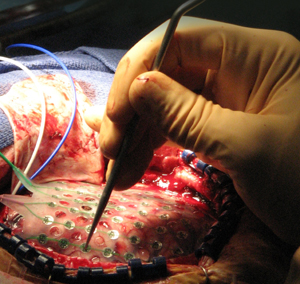
\includegraphics[width=0.4\textwidth]{img/bci1.jpg}
%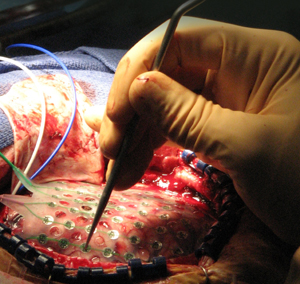
\includegraphics[scale=1,bb=0 0 30 30]{img/bci1.jpg}
\caption{BCI invasivo\cite{img:invasive-bci}} \label{fig:bci1}
\end{figure}

\item BCI semi invasivos: Son implantados dentro del cr�neo pero sin tocar la corteza cerebral. Producen una mejor se�al que los BCI no invasivos y tienen menor riesgo de causar da�os al cerebo que los BCI invasivos.

\item BCI no invasivos: Los implantes no invasivos son colocados en el cuero cabelludo. Los BCI no invasivos producen se�ales d�biles porque el cr�neo amortigua las se�ales, dispersando las ondas electromagn�ticas creadas por las neuronas.
\begin{figure}[htb]
\centering
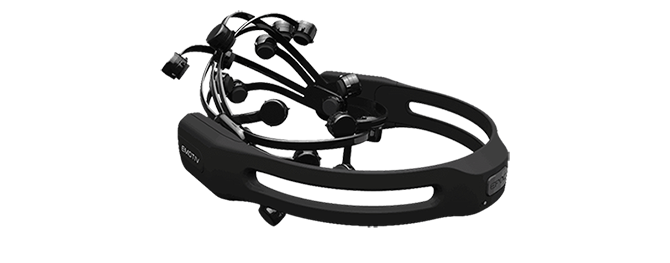
\includegraphics[width=0.8\textwidth]{img/epoc.png}
%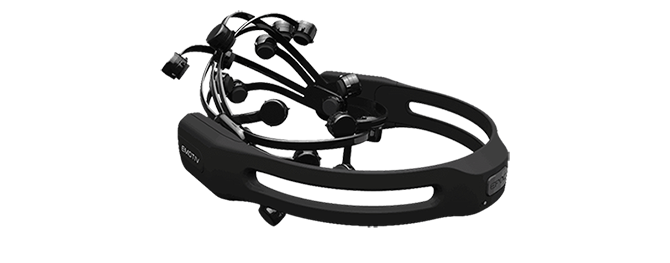
\includegraphics[scale=1,bb=0 0 30 30]{img/epoc.png}
\caption{BCI no invasivo\cite{emotiv:Online}} \label{fig:bci2}
\end{figure}

\end{itemize}

\subsection*{BCI Invasivos}
\markboth{\MakeUppercase{BCI Invasivos}}{}
\addcontentsline{toc}{subsection}{BCI Invasivos}

Los dispositivos BCI invasivos son implantados directamente en el cerebro y tienen la m�s alta calidad de se�ales de los BCI. Estos dispositivos son usados para recuperar funciones de personas con par�lisis. Los BCI invasivos son usados tambi�n para recuperar la vista conectando el cerebro a c�maras externas y para restaurar el uso de extremidades usando brazos y piernas rob�ticos controlados por el cerebro. Como todos los dispositivos que se encuentran instalados en la materia gris del cerebro este tipo de BI produce una calidad de se�ales muy alta pero son propensos a causar cicatrices en el tejido cerebral causando que las se�ales comiencen a volverse d�biles o incluso la p�rdida de las reacciones del cuerpo por contener un objeto desconocido en el cerebro\cite{invasiveBCI1}. \\
En las ciencias de la visi�n los implantes en el cerebro han sido usados para tratar la ceguera no cong�nita\footnote{Una enfermedad cong�nita es aquella que se manifiesta desde el nacimiento, ya sea por un trastorno ocurrido durante el desarrollo embrionario, durante el parto o como consecuencia de un defecto hereditario}. William Dobell es uno de los primeros cient�ficos que vienen trabajando con una interfaz cerebro para restaurar la vista como una investigaci�n privada. El implant� su primer prototipo en Jerry, un hombre que qued� ciego en su adultez en 1978. �l insert� un BCI de 68 electrodos en la corteza visual de Jerry y logr� producir la sensaci�n  de ver una luz. En 2012 el experimento fu� realizado en Jens Neumann donde Dobell utiliz� un implante m�s sofisticado que permiti� un mejor mapeo. Investigadores de la Universidad de Emory en Atlanta, dirigidos por Philip Kennedy y Roy Bakay fueron los primeros en instalar un implante en el cerebro de un ser humano que produce se�ales de alta calidad suficientes para estimular el movimiento\cite{invasiveBCI1}. \\
Thomas Navin Lal et al. en su art�culo \cite{invasiveBCI1} desarrollaron un BCI llamado Thought Translation Device (TTD) es cual usan para ayudar a comunicarse a pacientes con par�lisis los cu�les han perdido sus funciones cognitivas. Para poder usar el TTD los pacientes debieron aprender a regular a voluntad su Slow Cortical Potentials (SCP)\footnote{Se llaman SCP (o potenciales corticales lentos en espa�ol) a los cambios relacionados con los eventos de corriente continua lenta obtenidas con los EEG provenientes de los grandes conjuntos de c�lulas en la capa cortical superior\cite{SCP:Online}.}. El sistema entonces permite a su usuario escribir textos en la pantalla de una computadora o navegar en internet. El sistema sin embargo cuenta con dos desventajas: no todos los pacientes logran controlar su SCP adem�s la intensidad de la se�al es un poco baja y a un usuario bien entrenado requiere aproximadamente 30 segundos para escribir un caracter. % insertar imagen del articulo
\newpage\cleardoublepage



El Emotiv Epoc es BCI que fue creado con el prop�sito de ser un perif�rico para juegos en Windows, OS X y Linux\cite{Emotiv:Wiki:Online}, cuenta con 14 electrodos y funciona como dispositivo de entrada. En 2011 Kirill Stytsenko, et al.\cite{stytsenko2011evaluation} realizaron un an�lisis del Emotiv EPOC para la CogSci Conference. Emotiv EPOC es un BCI de bajo costo basado en la tecnolog�a EEG. Cuenta con 14 electrodos montados en una diadema inal�mbrica que se coloca sin esfuerzo y se conecta a la computadora. Originalmente fue creada para los juegos de computadora pero la ``research edition'' permite el acceso a los datos para su an�lisis lo que abre nuevas posibilidades a la ciencia para realizar nuevos experimentos o integrarlo a los ya existentes. En dicho estudio se someten a diferentes pruebas al Emotiv EPOC y al G-TEC\cite{G-TEC:Online}. Al compararlos se obtiene que la informaci�n en general es igual, pero la se�al es m�s clara e intensa en el G-TEC. Uno de los desaf�os encontrados es la creaci�n de software de grabaci�n para ambos dispositivos.
\\ Job Ram�n de la O Ch�vez en su tesis Interfaz Cerebro - Computadora para el Control de un Cursor Basado en Ondas\cite{intcerebro} plantea una interfaz que permita la comunicaci�n entre el usuario y la computadora, haciendo uso de sus ondas cerebrales, para el control de un cursor en pantalla mediante comandos obtenidos de las lecturas de un amplificador de ondas cerebrales.
\\ En EPOC-alypse Mind Controlled Car\cite{seniorepoc} plantean la construcci�n de de un carro de control remoto que es controlado por la mente usando el Emotiv EPOC. El proyecto fue desarrollado utilizando el SDK oficial del Emotiv EPOC.
\\ Asim Raza en SSVEP based EEG Interface for Google Street View Navigation\cite{raza2012ssvep} analiza los sistemas BCI y su aplicaci�n en el mundo real. Tambi�n desarrolla un prototipo interactivo que pueda ser controlado en un ambiente controlado para demostrar el funcionamiento de los sistemas BCI. Para el desarrollo decidi� utilizar el software libre OpenViBE para la adquisici�n y procesamiento de las se�ales.
\\ En ROS: an open-source Robot Operating System\cite{2009ros} se explica el uso de la plataforma ROS para el desarrollo de aplicaciones de rob�tica y resumen los objetivos filos�ficos de ROS en:
\begin{itemize}
\item Per-to-per
\item Basado en herramientas
\item Multilenguaje
\item Ligero
\item Gratuito y de C�digo Abierto
\end{itemize}
%ROS provee una capa de comunicaci�n estructura basada en Peer-to-peer, basado en herramientas, adem�s es multilenguaje, ligero, gratuito y de c�digo abierto.
En Things that twitter: social networks and the internet of things\cite{kranz2010things} utilizan ROS aplicado en las redes sociales. ROS permite intercambiar informaci�n por medio de servicios con mensaje de request y response definidos. La informaci�n es intercambiada por una arquitectura publish/suscribe donde los procesos permiten que sus datos est�n disponibles para que otros procesos puedan utilizarlos.

% Trabajos sobre cda tipo de BCI, enfatizar no invasivo.
% LIrbos, publicaciones etc que hablen sobre ellos.
% aplicacion en los videojuegos
% Avance de las compa�ias en el tema de los BCI
% Quienes han investigado sobre BCI
% Paises avanzados en el campo
% Campos con los que se relaciona\newpage\cleardoublepage

%\listofalgorithms
\listoffigures
\listoftables

\bibliography{bib/Bibliografia}\newpage\cleardoublepage

\end{document}